\chapter{Визуализация сложения сигналов с разной частотой}
\label{ch:chap4}

\begin{figure}[ht]
    \centering
    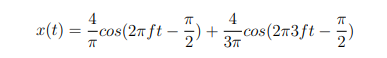
\includegraphics[width=1.0\textwidth]{diff_freq_1.png}
    \caption{Сложение двух сигналов разной частоты}
\end{figure}

В результате получим такую функцию:

\begin{figure}[ht]
    \centering
    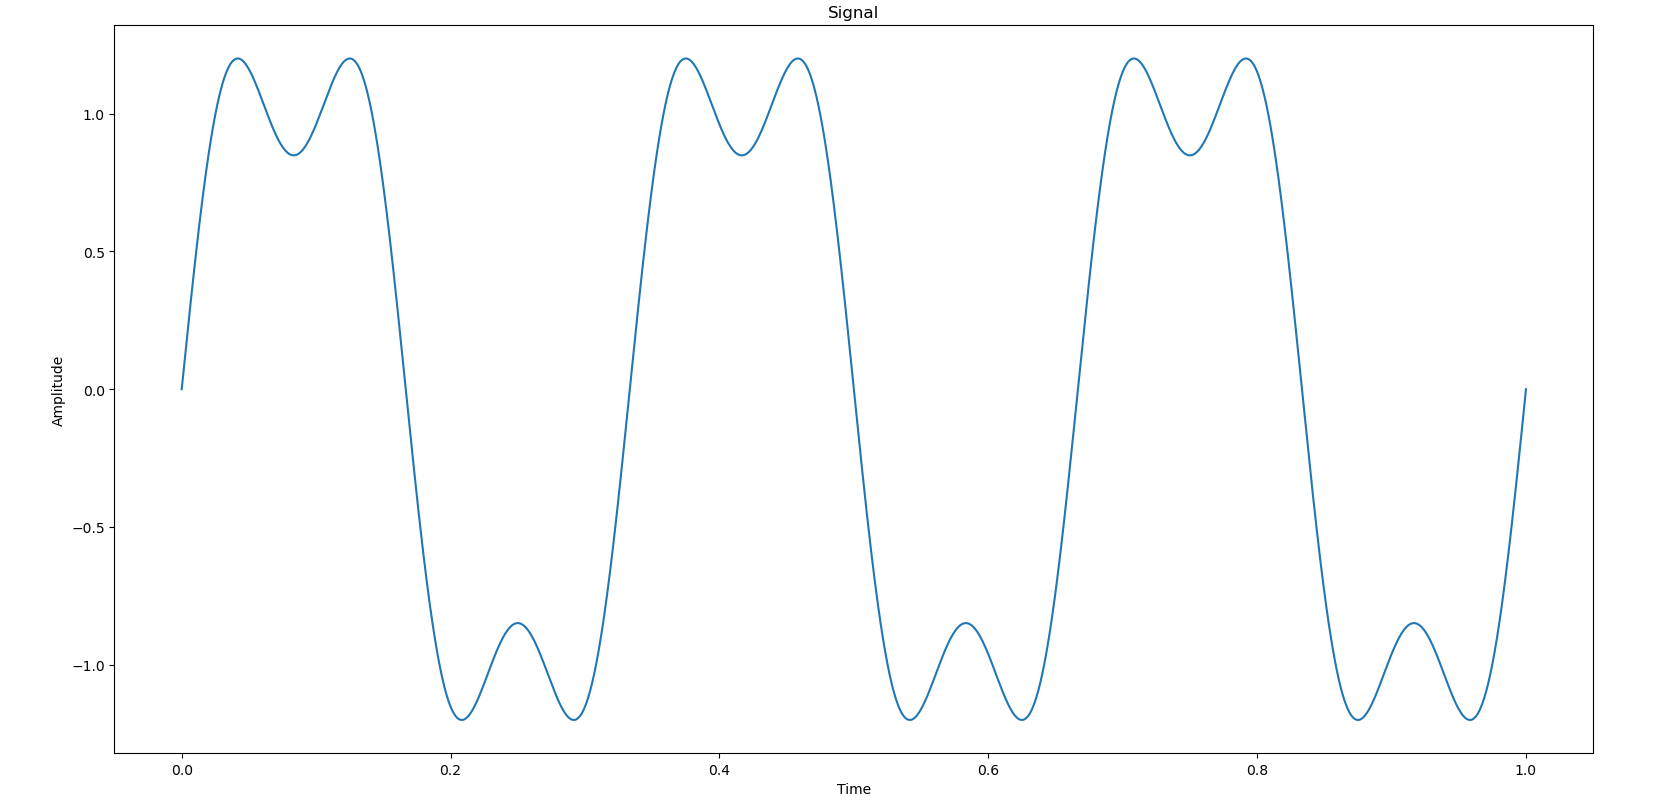
\includegraphics[width=1.0\textwidth]{multi_freq.png}
    \caption{Результат сложения сигналов разной частоты}
\end{figure}

Про этот сигнал нельзя однозначно сказать, какая у него частота, т.к в нем содержатся компоненты на 3Гц и 9Гц, и частота у сигнала переменная. \\

Просуммируем такие сигналы и визуализируем новый сигнал:

\begin{figure}[ht]
    \centering
    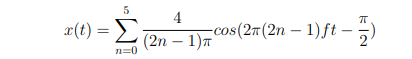
\includegraphics[width=1.0\textwidth]{diff_freq_2.png}
    \caption{Сложение N сигналов разной частоты}
\end{figure}

\begin{figure}[ht]
    \centering
    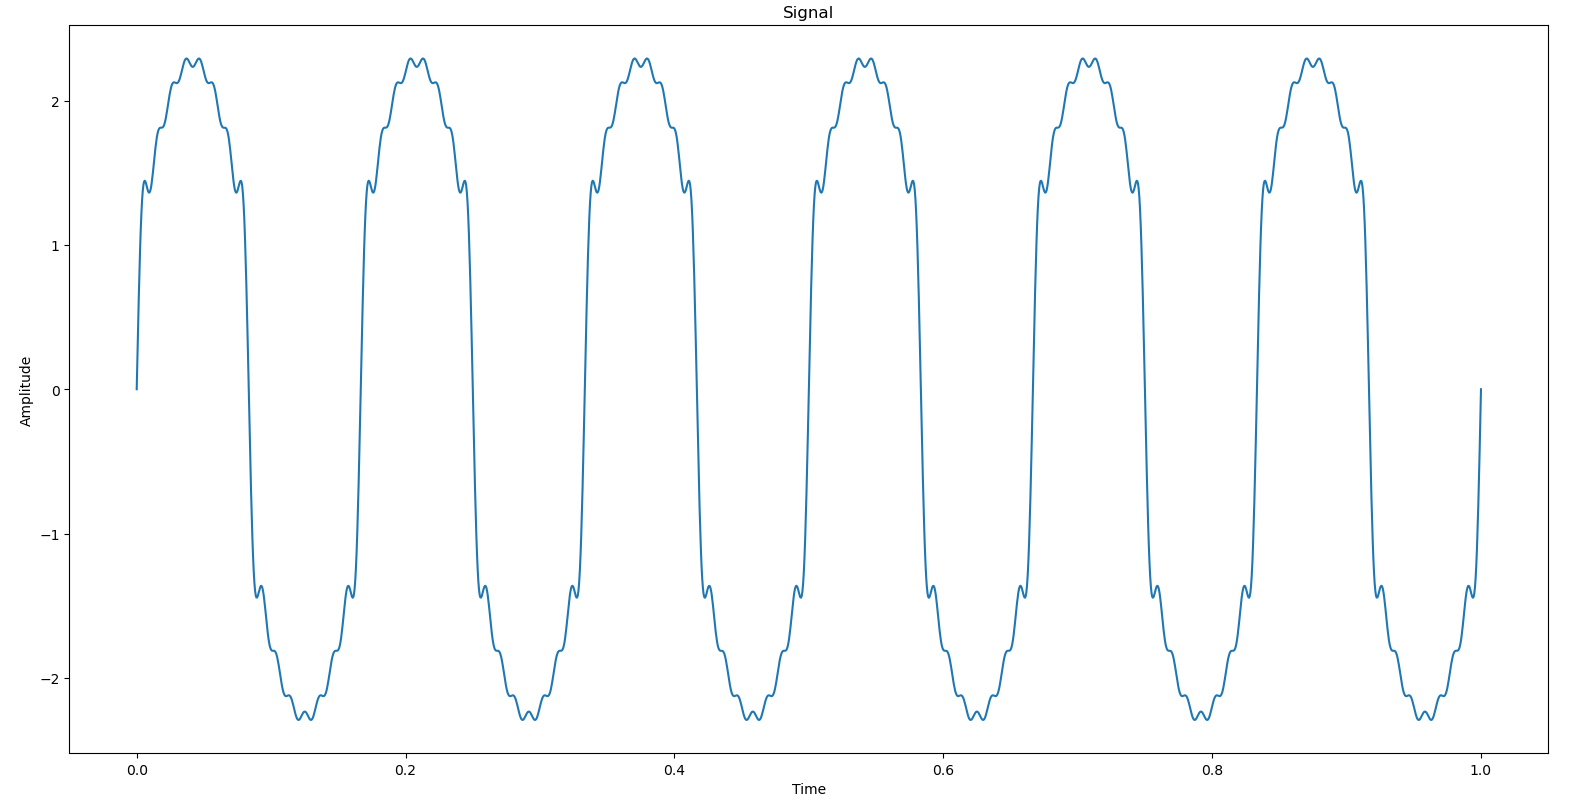
\includegraphics[width=1.0\textwidth]{multi_freq_2.png}
    \caption{Результат сложения N сигналов разной частоты}
\end{figure}




\endinput